For the sake of this demonstration, we have created a subset of the original data provided by the Amon Carter Museum of American Art that describes the artists behind the works the museum curates.  
To create a new source model for the ACMAA dataset in Karma, we first need to model the primary entity in the dataset, the artist.  To make the RDF for the dataset linkable, we need to create URIs for the artists.  
We do this by providing a few lines of Python to define a URI template using other fields to create a new field containing a URI for each artist.  We then model the artist by adding an E21\_Person to the source model.  
This creates a new node labelled E21\_Person1 and we set the URI of the node to the new field.  
We also create a E41\_Appelation with a rdfs:label to capture the artist's name.  
The new source model is illustrated in Figure~\ref{fig:simple-model-screenshot}. 


\begin{figure*}
\begin{center}
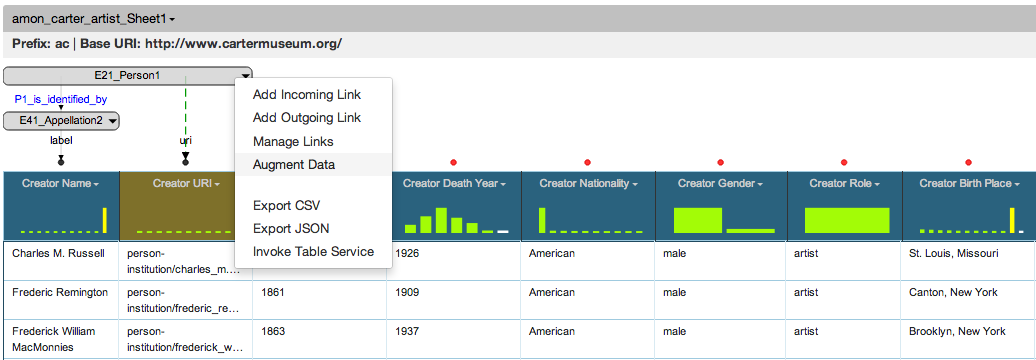
\includegraphics[width=4.8in]{images/4-simple-model.png}
\vspace{-3mm}
\caption{A simple model for describing an artist as an E21\_Person}
\vspace{-2mm}
\label{fig:simple-model-screenshot}
\end{center}
\vspace{-1.5em}
\end{figure*}




To facilitate the discovery and integration, we have also generated a set of owl:sameAs links between the artists in the new dataset and the artists from the Smithsonian dataset using LIMES \cite{ngomo2011limes}.
